%\setchapterimage{bandeau}
\chapter*{Application \arabic{cptApplication} \\ 
Mesure d'inertie -- \ifprof Corrigé \else Sujet \fi}
\addcontentsline{toc}{section}{Application \arabic{cptApplication} : Mesure d'inertie -- \ifprof Corrigé \else Sujet \fi}

\iflivret \stepcounter{cptApplication} \else
\ifprof  \stepcounter{cptApplication} \else \fi
\fi

\setcounter{question}{0}
\marginnote{Un classique ...}
\marginnote[1cm]{
\UPSTIcompetence[2]{C1-05}
\UPSTIcompetence[2]{C2-08}}


%\begin{marginfigure} [4cm]
%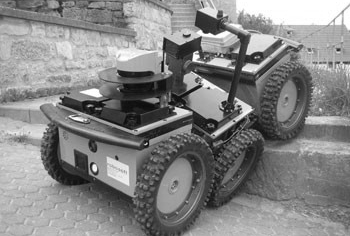
\includegraphics[width=\linewidth]{fig_00}
%\end{marginfigure}




\section*{Mise en situation}
La figure ci-contre représente un dispositif conçu pour déterminer le moment d’inertie d’un solide $S$ par
rapport à son axe de révolution matérielle, à partir de la mesure de la période de son oscillation sur deux
portées cylindriques d’un bâti $\Sigma$.

\begin{center}
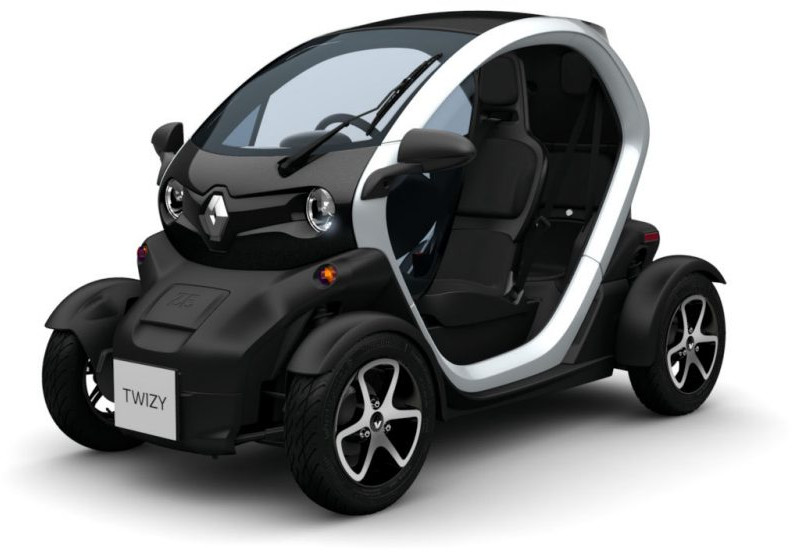
\includegraphics[width=.7\linewidth]{fig_01}
\end{center}
Soit $\repere{O}{x}{y}{z}$ un repère galiléen lié au bâti $\Sigma$. On désigne par $\vect{g}=g\vx{}$ l'accélération de la pesanteur. Les deux portées cylindriques de $\Sigma$ sont deux éléments de la surface cylindrique de révolution d’axe $\axe{O}{z}$, de rayon $r$ .
Le solide $S$ de masse $m$, de centre d’inertie $C$, possède deux tourillons de même rayon $a$ ( $a<r$ ).

L’étude se ramène à celle du problème plan suivant :
\begin{itemize}
\item le tourillon $S$, de centre $C$, roule sans glisser au point $A$ sur la portée cylindrique de $\Sigma$;
\item soit $\rep{1}\repere{O}{x_1}{y_1}{z}$ le repère, tel que le point $C$ soit sur l’axe $\axe{O}{x_1}$. $\theta=\angl{x}{x_1}$;
\item soit $\rep{2}\repere{C}{x_2}{y_2}{z}$ un repère lié à $S$. On pose $\varphi =\angl{x_1}{x_2}$. On suppose $\varphi=0$ lorsque $\theta=0$.
\end{itemize}
Notons $I$ le moment d’inertie de $S$ par rapport à son axe de symétrie $\axe{C}{z}$  et $f$ le coefficient de frottement entre $S$ et $\Sigma$.

On donne $a =\SI{12,3}{mm}$; $r =\SI{141,1}{mm}$; $ g = \SI{9,81}{m.s^{-2}}$; $m = \SI{7217}{g}$ ; $f = 0,15$.

\question{Déterminer la relation entre $\dot{\varphi}$ et $\dot{\theta}$.}

\question{Appliquer le théorème de l’énergie cinétique à $S$ dans son mouvement par rapport à $R$. En déduire
l’équation différentielle du mouvement sur $\theta$.}

\question{En supposant que l’angle $\theta$ reste petit au cours du mouvement, déterminer la période $T$ des
oscillations de $S$.}

\question{En déduire le moment d’inertie $I$ de $S$, sachant que $T=\SI{5}{s}$.}

En supposant toujours que l’angle $\theta$ reste petit, on pose $\theta=\theta_0\cos (\omega t)$ avec
$\omega = \sqrt{\dfrac{mg}{(r-a)\left(m+\dfrac{I}{a^2}\right)}}$.

On suppose à la date $t=0$, tel que $\theta = \theta_0$ et $\dot{\theta}=0$.

\question{Déterminer la valeur maximale de $\theta_0$ pour que $S$ roule sans glisser sur $\Sigma$.}

